\documentclass{../exhibit}

\title{Pirate Logic}

%% Font
\usepackage{imfellEnglish}
\usepackage[T1]{fontenc}
\raggedright

\usepackage{background}

\backgroundsetup{
scale=1,
color=black,
opacity=0.4,
angle=0,
contents={%
  \includegraphics[height=\paperheight]{mapBackground.jpg}%%https://upload.wikimedia.org/wikipedia/commons/8/81/Nautical_chart_of_the_West_Indies_1797.jpg
  }%
}




%% For the context
%% https://tex.stackexchange.com/questions/86150/torn-page-effect/86151#86151
\usepackage{tikz}
\usetikzlibrary{decorations.pathmorphing}
\definecolor{paper}{RGB}{239,227,157}





\renewcommand{\maketitle}{ %
  \begin{center}
    \scalebox{8}{\thetitle}
  \end{center}
  
\begin{tabular*}{\textwidth}{c @{\extracolsep{\fill}} c}  
\resizebox{4in}{!}{\begin{minipage}[b]{3in}\huge\directions\end{minipage}} &
  \resizebox{4in}{!}{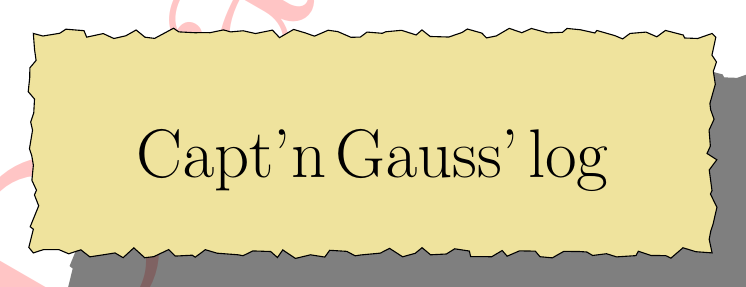
\begin{tikzpicture}[pencildraw/.style={ %
    decorate,
    decoration={random steps,segment length=4pt,amplitude=2pt}
    } %
]
\node[
preaction={fill=black,opacity=.5,transform canvas={xshift=.5cm,yshift=-.5cm}},
pencildraw,draw,fill=paper,text width=3in,inner sep=.5cm] 
{\begin{center}\Huge Capt'n Gauss' log \end{center}\vspace{.7cm} {\huge\context}};
\end{tikzpicture}}

\end{tabular*}

\vfill

\includegraphics[width=3in]{logoPirate.png}\hfill \includegraphics[width=2in]{bammLogo.png}


}



\begin{document}


\begin{context}
These \textsc{matrix riddles} were are boggling me brain.
\\[1cm]
Help me solve these mysteries of the sea!
\end{context}

\begin{directions}
  \begin{itemize}
  \item Use a grid to store information.
  \item The more information your record, the more you can deduce.
  \item Solve these puzzles by completing the banks in the grid.
  \end{itemize}
\end{directions}

\begin{example}
  \begin{center}
  \begin{tabular}{|>{\vphantom{X}}l|l|*{10}{A{\logpuzzlecellwidth}|}}
  \multicolumn{1}{c}{}  & \multicolumn{1}{c}{} & \multicolumn{5}{|c|}{Captains} & \multicolumn{5}{c|}{Ships} \tabularnewline[1ex]
  \cline{3-12}
\multicolumn{1}{c}{} & \multicolumn{1}{c|}{} & \rotatebox{90}{Artin} & \rotatebox{90}{Bourbaki} & \rotatebox{90}{Cauchy}  & \rotatebox{90}{DeMorgan} & \rotatebox{90}{Euler} & \rotatebox{90}{A} & \rotatebox{90}{B} & \rotatebox{90}{C}  & \rotatebox{90}{D} & \rotatebox{90}{E}  \tabularnewline
\hline
\multirow{6}{*}{\rotatebox{90}{Schooners}}  & A & & & & & & & & & & \tabularnewline
  \cline{2-12}
  & B & & & & & & & & & & \tabularnewline  
  \cline{2-12}
  & C & & & & & & & & & & \tabularnewline
  \cline{2-12}
  & D & & & & & & & & & & \tabularnewline
  \cline{2-12}
  & E & & X & & & & & & & & \tabularnewline
\hline
\multirow{6}{*}{\rotatebox{90}{Brigantines}}  & A & & & & & & \multicolumn{5}{c}{} \tabularnewline
  \cline{2-7}
  & B & & & & & & \multicolumn{5}{c}{} \tabularnewline
  \cline{2-7}
  & C & & & & & X & \multicolumn{5}{c}{} \tabularnewline
  \cline{2-7}
  & D & & & & & & \multicolumn{5}{c}{} \tabularnewline
  \cline{2-7}
  & E & & & & & & \multicolumn{5}{c}{} \tabularnewline
  \cline{1-7}
  \end{tabular}
  \end{center}
\end{example}

\begin{mathConnections}
  https://bartsnapp.github.io/Math-Outreach-Exhibits/matrixRiddles/
\end{mathConnections}
\end{document}
